%%%%%%%%%%%%%%%%%%%%%%%%%%%%%%%%%%%%%%%%%%%%%%%%%%%%%%%%%%%%%%%%%%
%%%%%%%%			BACKGROUND
%%%%%%%%%%%%%%%%%%%%%%%%%%%%%%%%%%%%%%%%%%%%%%%%%%%%%%%%%%%%%%%%%%

\section{Background \& Literature Review}

\subsection{Introductory Statement}

\paragraph{} 
Due to my personal experience working as a trainee electrical engineer for an electrical contractor I have a stronger understanding of power systems in the construction industry than most students at my level. This project will be focusing on a designs and simulations to produce deliverables.  

%%%%%%%%%%%%%%%%%%%%%%%%%%%%%%%%%%%%%%%%%%%%%%%%%%%%%%%%%%%%%%%%%%
%%%%%%%%			LITERATURE REVIEW
%%%%%%%%%%%%%%%%%%%%%%%%%%%%%%%%%%%%%%%%%%%%%%%%%%%%%%%%%%%%%%%%%%

\subsection{Literature Review}

\subsubsection{Existing Power Distribution Systems}

\paragraph{}
Power systems consist of four major sections; generation, transmission, distribution and loads. AC electricity is generated in power plants and sent through high voltage transmission lines to substations and distributed to switchboards for use in residential, commercial and industrial areas \cite{Amin2011}. In order to transport electricity over large distances (excess of 2km) without severe losses, very high voltage and low current is used \cite{Amin2011}. This is voltage is lowered and current increased by a transformer at the substation and again at the residence. For electricity to reach the home and be utilised for devices there must be safety mechanisms installed to ensure damage is not done to the user or devices. The protective devices requiring consideration throughout this project will be fuses, circuit breakers and switchboards \cite{UnitedStatesDepartmentoftheInterior2000}. These devices are placed through the circuit to protect the more expensive equipment closer to the transformer and grid.  

\begin{figure}[H]
\hfill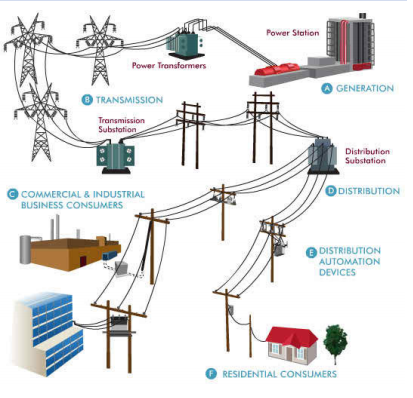
\includegraphics[width = 130mm]{images/Power_Distro}\hspace*{\fill}
\caption{Current Power Distribution Methods \cite{Active2015}}
\label{fig:CurrentPower}
\end{figure}    

\subsubsection{Alternative Electricity Generation Solutions}

\paragraph{}
In order to increase efficiency of power systems through utilising a low voltage DC sub-system, alternatives to drawing standard AC electricity from the grid must be considered. In Australia, a strong option for the generation alternative is photo-voltaic systems that are also known as solar panels. These systems will convert the sun’s rays into electricity via a DC-DC converter and a DC-AC inverter and battery \cite{Pillay2004}. An important aspect is that the electricity is produced in DC and will require no inverter in a DC system.

\subsubsection{Electrical Safety Mechanisms}

\paragraph{}

\subsubsection{Standards}

\paragraph{}
Australian standards will be an integral part of this project. Without adhering to the rules and regulations put in place, the devised system will not be legally allowed to be installed. There are three standards that will be relevant to this report; AS3000, AS3008 and AS3015. The AS/NZS 3000 covers the standards realted to electrical installations or wiring rules within Australia and New Zealand \cite{StandardsAustralia2007}. These standards will be the main reference point however there are the additional publications of AS/NZS 3008 which are the regulations specifically related to electrical installations and cable specifications \cite{StandardsAustralia2010}. The final standards taken into consideration will be AS/NZS 3015 which specifically disctates the rules with regards to electrical installations of extra low voltage direct current power supplies and services earthing within public telecommunications \cite{StandardsAustralia2004}.    

\subsubsection{Tariffs}

\paragraph{}
Tariffs will be an important considerion with the feasibility of this project due to the
possibilities of cost reduction. User expenses could theretically be reduced by imple-
menting a system off the grid. Government policies have been put in place in order
to prompt an increase in investment in renewable energy sources \cite{Nelson2011}. Users are able to sell their unused generated electricity back to the grid to reduce their overall electricity
bills or possibly profit if consumption is low enough. In Queensland, according to the
SolarChoice website a feed-in tariff of \$0.06/kWh can be earned \cite{website:SolarChoice}. By not connecting the photo voltatic panels to the grid, this tariff can not be received however there is the possibility that it is more efficient and will produce less energy loss by storing in local
batteries and running simple circuits rather than feeding the grid \cite{AntoniouATzimasARowland2015}. The consideration will be whether the cost reduction in electricity bill will be worth the investment in the equipment and future cost reduction.   

\subsubsection{Direct Current vs Alternating Current}

\paragraph{}
A very broad and contextual understanding must be made about the differences be-
tween direct current and alternating current distribution systems. Compared with tradi-
tional AC designs, DC has the potential for large power supply capacity, smaller feeder
loss, increased efficiency, more consistent power and more direct access to renewable
energy solutions \cite{Liu2014}. Alternating current is run to outlets at 240V, 50Hz and then
devices are used to alter that source into whatever the device requires. Many house-
hold electronics such as computers, chargers, lighting and televisions operate internally
at DC voltages meaning they each require either internal conversion circuitry or use a
transformer between the powerpoint and device \cite{Paajanen2009}.

\paragraph{}
AC was originally depicted as the better choice for power distributions due to there
being no method at the time for controlling DC electricity at the load causing large
losses from the generator to device \cite{Starke2008b}. To remedy this, AC distribution was used
due to efficienct transformers being developed to boost the voltage. AC remains the
fundamental power type but DC is growing in popularity with improved converters and
increased frequency of DC energy sources \cite{Starke2008b}. Utilising DC generation systems could
also fulfill the power industry’s obligation to increase the sustainability of their systems
and be more environmentally conscious \cite{Starke2008a}. The required inverters to convert the AC
supply into DC for electronics is reducing the efficiency (increasing voltage drop) of the
overall system \cite{Starke2008b}. 

\subsubsection{Direct Current \& Alternating Current}

\paragraph{}
A very broad and contextual understanding must be made about the differences between direct current and alternating current distribution systems. Compared with traditional AC designs, DC has the potential for large power supply capacity, smaller feeder loss, increased efficiency, more consistent power and more direct access to renewable energy solutions \cite{Liu2014}. Alternating current is run to outlets and devices are used to change the source for the device. Many household electronics such as computers, chargers, lighting and televisions operate internally at DC voltages meaning they each require either internal conversion circuitry or use a transformer between the powerpoint and device \cite{Paajanen2009}. Utilising DC generation systems could fulfill the power industry's obligation to increase the sustainability of their systems and be more environmentally conscious \cite{Starke2008a}. The required inverters to convert the AC supply into DC for electronics is reducing the efficiency of the overall system \cite{Starke2008b}.       

\subsubsection{Low Voltage Direct Current}

\paragraph{}
DC power is currently restricted to special applications such as telecommunications, electric vehciles and high-voltage direct current (HVDC) transmission \cite{Salomonsson2007}. Low-voltage DC power systems at 48V has been used fairly widely with telecommunications systems but is recently facing issues due to the high power requirements of computer system upgrades \cite{Salomonsson2007}. Studies have shown that the 48V system still remains more efficienct than a 270V DC or 200V AC but further investigation needs to be done into 230V and 325V through retrofitting existing low voltage AC installations \cite{Salomonsson2007}. Photo-voltatic generators are used frequently for these forms of power distribution systems as it can be powered directly or use simple DC to DC converters for different devices. Utilising a DC distribution system makes it easier to incorporate the local generation meaning not only could this be cheaper but if there are faults with the distribution grid, the separate micro-grid will be protected \cite{Starke2008a}. 

\subsubsection{Converters and Inverters}

\paragraph{}
Converters and inverters are electrical devices designed and constructed to convert
current \cite{website:ConvVsInverter}. Converters are used to convert the voltage from AC to DC and inverters converter from DC to AC \cite{website:ConvVsInverter}. Inverters are used to convert the DC from solar panels to AC for transfer back into mains or to the necessary switchboard. An additional use for these is in Uninterrupted Power Supplies (UPS) where stored DC battery power \cite{website:ConvVsInverter}. There are three different types of converters and inverters;

Converters \cite{website:ConvVsInverter}
\begin{itemize}[noitemsep]
\item Analog-to-digital converter (ADC): converts the input analog voltage to a digital
value proportional to the magnitude of the voltage or current. An example of these
would be a rotary encoder.
\item Digital-to-analog converter (DAC): converts digital code to an analog signal. An
example would be a computer sound card or digital music players.
\item Digital-to-digial converter (DDC): converts one form of digital data to another.
\end{itemize}

Inverters \cite{website:ConvVsInverter}
\begin{itemize}[noitemsep]
\item Square wave inverter: built from a DC source with four switches and a load, it
produces a square wave output. This is the cheapest device but produces the
lowest quality power.
\item Quasi wave or modified square wave inverters: the output waveform is square and
therefore not sine which is required for pure AC sine waves. These waves have
a step between the square waves which can aid in minimising noise or harmonics
that can cause problems with electrical devices.
\item  True sine wave inverters: the most expensive form of inverter. These are not used
actively due to the second option being more cost efficient.
\end{itemize}

\subsubsection{LED Lighting}

\paragraph{}
Improvements in LED lighting allow much less power to be used for the same amount of light. It is very possible to design and create an energy efficient LVDC grid powered LED lighitng system with additional automation aspects and energy storage \cite{Koh2011}. Typical lighting systems that are used in a lot of commercial or residential buildings are flurescent systems that are powered directly from standard 230V AC due to the devices' high efficacy \cite{Koh2011}. When comparing an AC flurescent system and a LVDC LED system, the LVDC gid system requires sigificantly less power conversion which increases the overall effiency \cite{Koh2011}. The image below additionally compares how lower wattage and power consumption is now able to produce far more light (lumens). This is allow fewer a similar amount of lights per room but they draw far less power \cite{website:LED}.  

\begin{figure}[H]
\hfill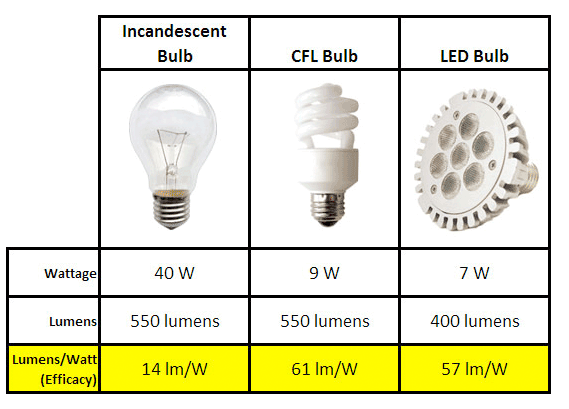
\includegraphics[width = 110mm]{images/LED_Comparison}\hspace*{\fill}
\caption{Comparing Lighting Method's Efficiency \cite{website:LED}}
\label{fig:LightingEfficiency}
\end{figure}
\newpage

\subsubsection{Commercial and Industrial Power Systems}

\paragraph{}
There are relatively large differences between home power systems and commercial. A home setting is fairly simple wih a transformer close to the house feeding the power into one switchboard that provides additional safety along with circuit breakers for the home circuits. In a commercial setting the loads are far higher and requires a stable connection \cite{Baran2003}. For an apartment complex, shopping centre or business building for example, the supplies are usually separated into busses in order to identify separate requirements or areas. The requirements could be essential items (including emergency lifts, safety equipment or machines that cannot be stopped) or non-essentials (tenancies or general equipment). Additionally it can be used to separate the entire building's load over towers or zones to minimise faults. The figure below represents a single line diagram showing the two separate busses for a design. 

\begin{figure}[H]
\hfill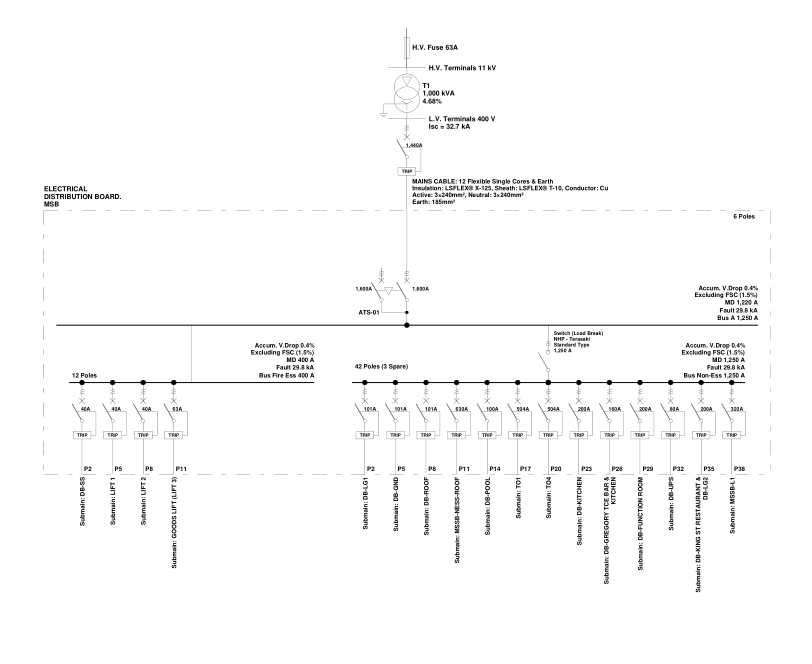
\includegraphics[width = 160mm, height = 110mm]{images/PCad_SLD}\hspace*{\fill}
\caption{{Hotel Single Line Diagram}}
\label{fig:SLD}
\end{figure}   

\subsubsection{Buck and Boost Converters}

\paragraph{}

\newpage